\section{Understanding User Data Deletion Practices and Expectations}
\label{sec:user_study}

To investigate users' data deletion practices and expectations in LLM agents (RQ1 and RQ2), we conducted an online survey of users with prior experience deleting data from LLM agents.
%
This section describes our study methodology and presents the key findings.

\subsection{User Study Methodology}

\subsubsection{Participant Recruitment}
%
We recruited participants through Prolific, targeting adults aged 18 or older residing in the United States who had used at least one of the six LLM agents described in Section~\ref{sec:background}. 
%
The survey was administered through Qualtrics, with a recruitment target of approximately 200 participants to support the exploratory nature of the study.
%
Participants received \$4 upon completing the survey and passing the attention checks.
%
Of 235 submissions, we excluded 36 participants who reported no prior experience deleting data from LLM agents, as our analysis focused on users with such experience. 
%
We further excluded 17 incomplete submissions, one response that failed an attention check, and four participants with missing responses to key survey questions, yielding a final sample of 177 participants.
%
Among these participants, 58.8\% were men, 40.7\% were women (one preferred not to say), 73.4\% were under 45 years old, and 62.1\% held at least a bachelor's degree (Table~\ref{tab:demographics}). 
%
Thus, our survey findings characterize users with prior deletion experience rather than the broader population of LLM-agent users.
%
Separately, we collected deletion-request prompts from 209 participants, including some without prior deletion experience, for the later post-deletion analysis in Section~\ref{sec:didr}, as the hypothetical prompt-writing task did not require such experience.
%
Table~\ref{tab:demographics} in the Appendix presents the demographic details of the participants.

\subsubsection{Study Procedure}
%
The survey was designed to take about 15 minutes to complete. 
%
Participants first reviewed an informed consent form describing the study's purpose, procedures, data handling, and participant rights. 
%
Those who consented proceeded to screening questions assessing their age, U.S. residence, and prior use of LLM agents.
%
Eligible participants then completed the following survey components in sequence: (1) LLM-agent usage and prior use of deletion methods; (2) scenario-based assessments of deletion practices, expectations, and verification; (3) prior data deletion experiences; (4) deletion feedback and desired confirmation mechanisms; (5) privacy awareness and knowledge; (6) attitudes toward LLM agents, data sharing, social influences, and perceived AI-related abilities; and (7) demographic information.
%
The scenario-based assessments involved two scenarios presented in randomized order, each followed by the same set of questions. 
%
Two instructed-response attention checks were embedded in the survey to assess response quality. Throughout the survey, we used the term ``AI chatbot'' to refer to LLM agents, as this term is more familiar and accessible to general users.

\subsubsection{Survey Question Design}
%
\label{subsubsec:questions}
%
We designed the survey questions to investigate users' deletion practices (RQ1) and their expectations and verification strategies (RQ2), using scenario-based assessments complemented by questions about prior experiences.

\para{Scenario design}
%
To investigate users' deletion practices and how these practices vary across different contexts, we developed two hypothetical scenarios involving different levels of data sensitivity and usage contexts.
%
The less sensitive scenario (\textbf{LS}) concerns sharing a city while requesting weather information, whereas the more sensitive scenario (\textbf{MS}) concerns disclosing a home address while seeking a clinic for sexually transmitted infection treatment.
%
In both scenarios, participants were asked to consider deleting the disclosed location information to protect their privacy. 
%
The scenarios used identical follow-up questions and were presented in randomized order to enable within-participant comparisons while mitigating potential order effects.

\para{Data deletion practices (RQ1)}
%
Before evaluating the scenarios, participants were introduced to eight deletion methods, including the six methods described in Table~\ref{tab:methods}, account deletion, and filing a deletion request.
%
Each method was accompanied by a description and example screenshot. 
%
Participants reported which methods they had previously used.
%
For each scenario, participants selected a deletion method from those they had previously used and explained their choice. 
%
They then rated the selected method along three dimensions using five-point agreement scales: \textit{perceived privacy protection} (five items), \textit{effort} (four items), and \textit{potential loss of personalized benefits} (three items). 
%
Participants also indicated their willingness to delete the disclosed information on a five-point scale. 
%
Finally, they selected their preferred deletion methods from all available options, regardless of prior experience, allowing us to distinguish prior method use from hypothetical preferences.

\para{User expectations and verification (RQ2)}
%
For each scenario, participants indicated what they expected their selected deletion method to accomplish, including \textit{permanent deletion from the database and backups}, being \textit{made invisible to users}, the agent not referencing the information in \textit{the current conversation} or in \textit{future conversations}, and \textit{exclusion from model training}. 
%
Participants could select multiple outcomes or indicate uncertainty.
%
We also asked participants how they had previously verified deletion, including asking the agent in the same or a new conversation, checking saved memories or the user interface, and submitting a data access request through a privacy portal. 
%
Participants could indicate that they did not know how to verify deletion or did not wish to do so, and rated their confidence in verification. 
%
Additional questions examined the confirmation participants had received after previous deletion attempts and the feedback they believed LLM agents should provide.

\para{Participant-authored deletion-request prompts}
%
In each scenario, participants wrote the message they would send to an LLM agent to request deletion of the disclosed information and explained their wording. 
%
These participant-authored deletion-request prompts were later used as inputs to our post-deletion analysis (RQ3; Section~\ref{sec:didr}), allowing us to evaluate LLM agents using prompts written by survey participants (i.e., real users).

\para{Other survey questions}
%
We also asked participants about their prior deletion experiences, including the types of information they had attempted to delete, their motivations, how they discovered deletion controls, and whether agents had subsequently referenced information they believed was deleted.
%
Finally, we collected participants' demographic characteristics, including education level, gender, and primary domain of work or study. 
%
To assess response quality, we also embedded two instructed-response attention checks in the survey, asking participants to select a specific response option to verify that they were reading and following the instructions carefully.
%
The complete questionnaire, including question wording and measurement items, is provided in Appendix~\ref{app:questions}.


\subsubsection{Data Analysis}
%
We analyzed responses from 177 participants, reporting percentages separately for the less sensitive (LS) and more sensitive (MS) scenarios. 
%
Because each participant evaluated both scenarios, we used paired statistical tests to compare their responses. 
%
Specifically, we used Wilcoxon signed-rank tests~\cite{wilcoxon1945individual} for \textit{willingness to delete}, \textit{perceived privacy protection}, \textit{effort}, and \textit{benefit loss}; the Stuart-Maxwell test~\cite{agresti2013categorical} for overall deletion-method choices; and McNemar tests~\cite{agresti2013categorical} for individual deletion methods, expected deletion outcomes, and verification strategies. 
%
We also examined potential scenario-order effects using binomial~\cite{agresti2013categorical}, Mann-Whitney~\cite{mann1947test}, and Fisher's exact tests~\cite{agresti2013categorical}. 
%
To compare deletion methods, we pooled responses from both scenarios (\textbf{Pooled}), with each participant contributing two responses. 
%
We fitted generalized estimating equations (GEE)~\cite{liang1986longitudinal} clustered by participant to account for within-participant dependence. 
%
To avoid unstable estimates from small groups, we restricted these analyses to the four deletion methods selected by at least 14 participants, retaining 317 of the 354 responses. 
%
We used Gaussian models~\cite{liang1986longitudinal} for \textit{perceived privacy protection}, \textit{effort}, and \textit{benefit loss}, and logistic models~\cite{agresti2013categorical} for binary expectation outcomes, with scenario included as a covariate. 
%
Pairwise differences in effort were assessed using GEE contrasts, while verification strategies were compared across methods using chi-square or Fisher's exact tests separately for each scenario.


We assessed the three perception scales using confirmatory factor analysis (CFA), with separate factors for protection (five items), effort (four items), and benefit loss (three items).
%
Standardized factor loadings ranged from .73 to .94, average variance extracted from .64 to .76, and Cronbach's $\alpha$ from .87 to .92. Model fit was acceptable on several indices (CFI = .94, TLI = .92, SRMR = .060), although RMSEA = .099 exceeded the conventional .08 threshold. 
%
Because the pooled CFA did not account for repeated responses, we also fitted separate models for each scenario, obtaining similar results (CFI = .95 and .93; RMSEA = .087 and .108). 
%
We treated the analyses as exploratory and applied Holm corrections~\cite{holm1979simple} within families of related tests, leaving individual tests unadjusted. 
%
We report adjusted values as $p_{\mathrm{Holm}}$. 
%
Table~\ref{tab:analysis-families} summarizes the statistical tests, sample sizes, and correction families.

\begin{table*}[t]
\centering
\caption{Summary of statistical analyses, tests, and multiple-testing correction families.}
\label{tab:analysis-families}
\small
\begin{tabular}{@{}p{0.32\textwidth}p{0.28\textwidth}p{0.20\textwidth}p{0.14\textwidth}@{}}
\toprule
Analysis & Statistical test & Sample & Holm family \\
\midrule

\multicolumn{4}{@{}l}{\textit{Scenario comparisons (LS vs. MS)}} \\
Willingness to delete
    & Wilcoxon signed-rank; rank-biserial $r$
    & 177 pairs
    & None (single test) \\
Protection, effort, and benefit loss
    & Wilcoxon signed-rank; rank-biserial $r$
    & 177 pairs
    & 3 scales \\
Deletion-method choice (overall)
    & Stuart-Maxwell marginal homogeneity
    & 176 participants who chose a method in both scenarios
    & None (single test) \\
Deletion-method choice (each method)
    & McNemar
    & 177 participants
    & 7 methods \\
Expected deletion outcomes
    & McNemar
    & 177 participants
    & 7 options \\
Verification strategies
    & McNemar
    & 177 participants
    & 8 options \\
\midrule

\multicolumn{4}{@{}l}{\textit{Deletion-method comparisons}} \\
Protection, effort, and benefit loss
    & Gaussian GEE, clustered by participant (Wald)
    & 317 responses, 4 methods
    & 3 scales \\
Effort (pairwise between methods)
    & GEE contrasts, adjusted for scenario
    & 317 responses, 4 methods
    & 6 method pairs \\
Expected deletion outcomes
    & Logistic GEE, clustered by participant
    & 317 responses, 4 methods
    & 7 options \\
Verification strategies
    & Chi-square or Fisher's exact, each scenario separately
    & Participants choosing a method with at least 14 participants in that scenario
    & 8 options, within each scenario \\
\midrule

\multicolumn{4}{@{}l}{\textit{Measurement validation and robustness checks}} \\
Scale structure
    & Confirmatory factor analysis
    & 354 responses
    & Not applicable \\
Scenario order
    & Binomial test, Mann-Whitney, Fisher's exact
    & 177 participants
    & 4 ratings (Mann-Whitney) \\
\bottomrule
\end{tabular}

\par\vspace{0.5em}
\begin{minipage}{0.94\textwidth}
\footnotesize
\textit{Note.} LS and MS denote the less and more sensitive scenarios, respectively.
A response is one participant's answer in one scenario.
GEE denotes generalized estimating equations.
Holm corrections are applied within the specified families;
single tests are not adjusted.
\end{minipage}
\end{table*}

\subsection{User Study Findings}
\label{sec:qual_results}

We present findings from 177 participants, organized around users' deletion practices (RQ1) and their expectations and verification strategies (RQ2).
%
Results are reported separately for the less sensitive (LS) and more sensitive (MS) scenarios.
%
Analyses combining both scenarios are denoted as \textbf{Pooled}, comprising 354 responses unless otherwise specified.

\subsubsection{User Deletion Practices (RQ1)}

Deleting a single conversation was the most commonly used deletion method (76.8\% of participants) and the most frequently selected method in both scenarios (Table~\ref{tab:method-use}).
%
Clearing all conversation history was also common (53.1\%), whereas deleting a specific saved memory (32.2\%) and clearing all saved memories (25.4\%) were less frequently reported.
%
Fewer participants had used a privacy dashboard (9.6\%), deleted their account (10.2\%), or filed a deletion request (2.8\%).
%
Most participants discovered deletion controls by exploring the settings or guessing how to delete their data, while only 6 of 177 reported learning about these options from the agent itself.

\begin{table*}[!t]
\centering
\caption{Previously used deletion methods (multiple selections allowed) and scenario-based method choices in LS, MS, and Pooled. Scenario-based choices were restricted to methods participants had previously used; ``Other'' choices are excluded from the pooled counts.}
\label{tab:method-use}
\small
\begin{tabular}{@{}lrrrr@{}}
\toprule
 & Previously used & \multicolumn{3}{c}{Chosen in scenario} \\
\cmidrule(lr){3-5}
Deletion method & ($n=177$) & LS & MS & Pooled ($n=352$) \\
\midrule
Sending a deletion-request prompt & 55 (31.1\%) & 25 & 14 & 39 (11.1\%) \\
Deleting a single conversation & 136 (76.8\%) & 84 & 80 & 164 (46.6\%) \\
Clearing all conversation history & 94 (53.1\%) & 33 & 40 & 73 (20.7\%) \\
Deleting a specific saved memory & 57 (32.2\%) & 19 & 22 & 41 (11.6\%) \\
Clearing all saved memories & 45 (25.4\%) & 7 & 8 & 15 (4.3\%) \\
Using a privacy dashboard & 17 (9.6\%) & 6 & 9 & 15 (4.3\%) \\
Deleting the account & 18 (10.2\%) & 2 & 3 & 5 (1.4\%) \\
Filing a request & 5 (2.8\%) & 0 & 0 & 0 (0.0\%) \\
\bottomrule
\end{tabular}
\end{table*}

The more sensitive scenario increased participants' willingness to delete the disclosed information, but did not significantly change their deletion-method choices.
%
In LS and MS, respectively, 125 and 150 of 177 participants indicated that they would probably or definitely delete the information.
%
Mean willingness increased from 3.98 in LS to 4.37 in MS on the five-point scale (Wilcoxon signed-rank test, $p<.001$, $r=.55$).
%
However, the overall distribution of deletion-method choices did not differ significantly between scenarios (Stuart-Maxwell test, $p=.39$, 176 participants).
%
Thus, although participants expressed greater willingness to delete information in the more sensitive scenario, we found no corresponding evidence of a change in their selected deletion methods.

Participants' preferred deletion methods also differed from their scenario-based choices.
%
Sending a deletion-request prompt was the second most frequently preferred method (47\%--50\% across LS and MS), following deleting a single conversation (61\%--66\%).
%
However, only 8\%--14\% of participants selected a deletion-request prompt from the methods they had previously used.
%
This gap suggests that deletion-request prompts appealed to many participants, even though relatively few had previously used them.

\begin{takeawaybox}
\textbf{Finding 1:} Participants primarily used conversation-level deletion methods and often discovered deletion controls on their own. The more sensitive scenario increased willingness to delete but did not significantly change deletion-method choices. Although many participants preferred deletion-request prompts, relatively few selected them among their previously used methods.
\end{takeawaybox}


\subsubsection{User Expectations and Verification (RQ2)}

Participants expressed similar expectations across deletion methods, despite differences in the data locations these methods target.
%
Across Pooled responses, 59.0\% expected permanent deletion from the agent's databases and backups, while 54.2\% expected the information to become unavailable for recall in future conversations (Figure~\ref{fig:expectation}).
%
Among the four most frequently selected methods, we detected no statistically significant differences in expectations of permanent deletion ($p_{\mathrm{Holm}}=1.0$) or prevention of recall in future conversations ($p_{\mathrm{Holm}}=1.0$).
%
These results suggest that participants did not consistently distinguish deletion methods by their expected outcomes.
%
In contrast, participants perceived differences in the effort required by deletion methods.
%
Among the four most frequently selected methods, perceived effort differed significantly ($p_{\mathrm{Holm}}=.0001$), whereas perceived privacy protection did not ($p_{\mathrm{Holm}}=.29$; Figure~\ref{fig:scales}).
%
These results suggest that participants differentiated methods more by perceived effort than by expected protection.
%
However, because participants selected their own methods and the groups were relatively small, these comparisons are associative rather than causal.

\begin{figure}[t]
    \centering
    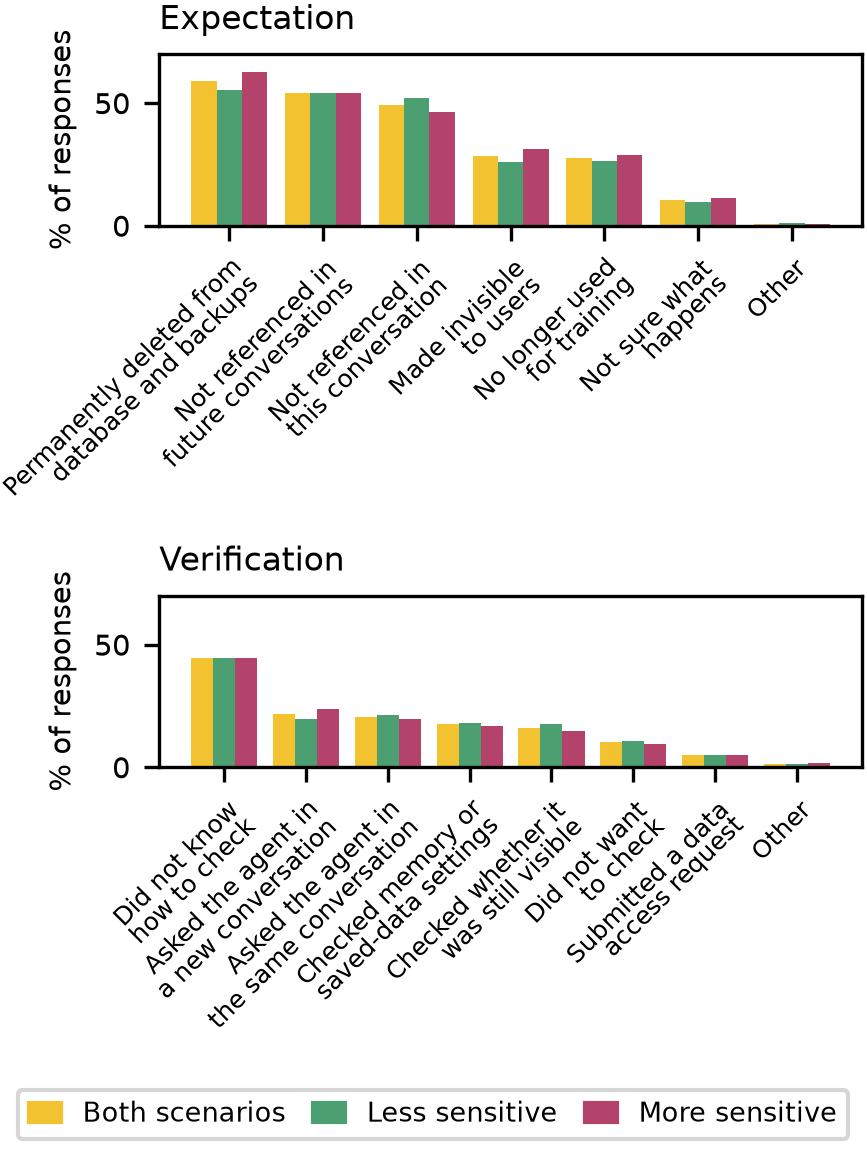
\includegraphics[width=\columnwidth,height=0.42\textheight,keepaspectratio]{figures/fig_expectation.png}
    \caption{Expected deletion outcomes and reported verification strategies in LS, MS, and Pooled. The analysis includes 354 responses from 177 participants, with multiple selections allowed. Percentages are based on 177 participants within each scenario and 354 responses for Pooled results.}
    \label{fig:expectation}
\end{figure}


\begin{figure*}[t]
    \centering
    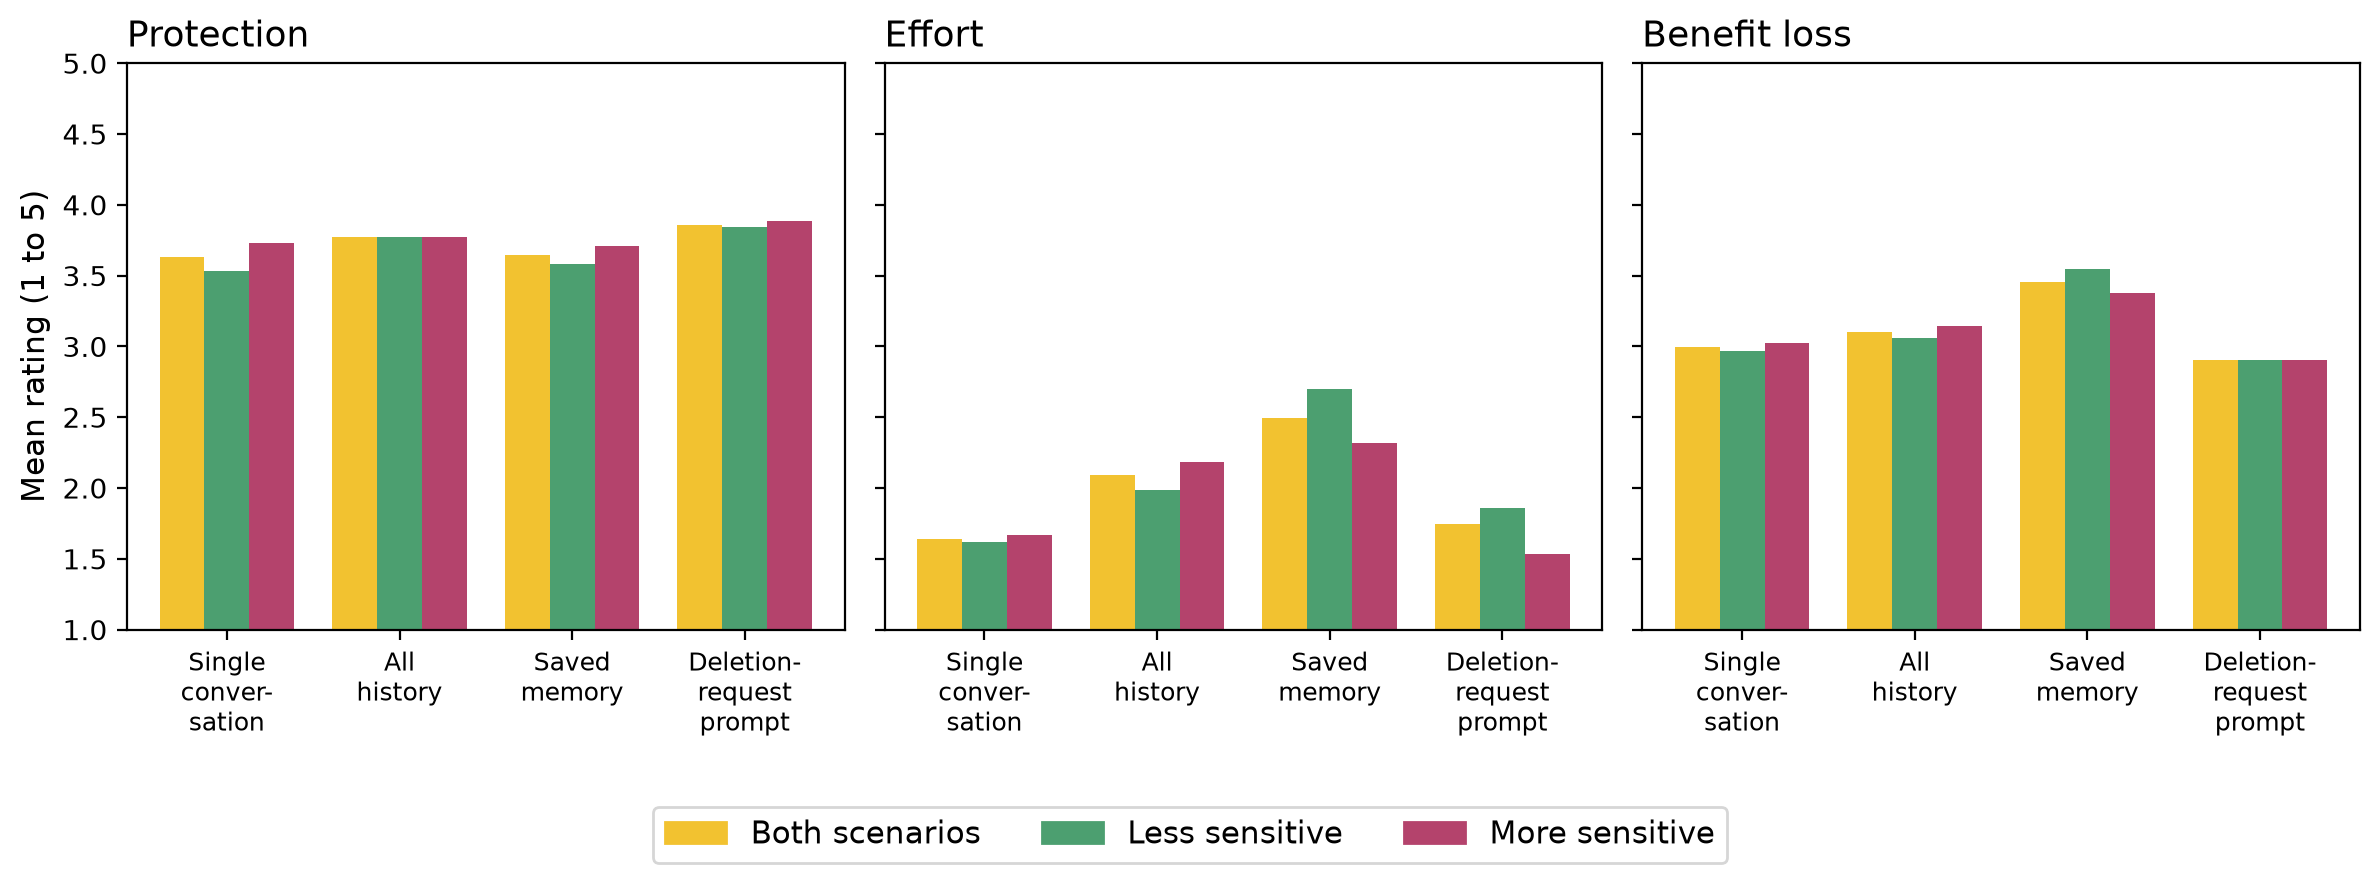
\includegraphics[width=0.9\textwidth]{figures/fig_scales.png}
    \caption{Mean ratings of perceived privacy protection, effort, and potential loss of personalized benefits for the four most frequently selected deletion methods, shown separately for LS and MS and combined (Pooled). The analysis includes 317 responses from 105, 50, 30, and 29 participants, respectively. Ratings use five-point agreement scales.}
    \label{fig:scales}
\end{figure*}

Many participants were uncertain how to verify deletion outcomes.
%
Across Pooled responses, 44.6\% indicated that they did not know how to verify deletion.
%
Reported verification strategies included asking the agent in the same or a new conversation (21\%--22\% of responses) and checking saved memories, settings, or the user interface (16\%--18\%).
%
Notably, among responses selecting a deletion-request prompt, 53.8\% (of 39 responses) indicated verification by asking the agent in the same conversation.
%
This suggests that users relying on conversational deletion requests may also rely on the agent's own responses as evidence that deletion succeeded.

Participants also reported limitations in deletion feedback and experiences of information resurfacing.
%
Among the 177 participants, 42 (23.7\%) reported that an agent had referenced information they believed was deleted.
%
After previous deletion attempts, 41.2\% reported receiving a clear confirmation message, while 29.4\%--34.5\% reported vague acknowledgements or no feedback (multiple selections allowed).
%
Furthermore, 73 participants (41.2\%) wanted a breakdown specifying what information had been deleted and what might still be retained.
%
These findings highlight a gap between users' expectations of deletion and their ability to establish its outcome, motivating our subsequent post-deletion analysis (Section~\ref{sec:tech_analysis}).

%
\begin{takeawaybox}
\textbf{Finding 2:} Participants commonly expected deletion methods to permanently remove their data, despite differences in the data locations these methods target. Perceived effort differed across methods, but expected deletion outcomes and perceived protection showed no significant differences. Many participants did not know how to verify deletion, and those selecting deletion-request prompts often relied on the agent itself for verification.
\end{takeawaybox}












% \section{Understanding User Data Deletion Practices and Expectations}
% \label{sec:user_study}

% To investigate users' data deletion practices and expectations in LLM agents (RQ1 and RQ2), we conducted an online survey of users with prior experience deleting data from LLM agents.
% %
% This section describes our study methodology and presents the key findings.

% \subsection{User Study Methodology}

% \subsubsection{Participant Recruitment}
% %
% We recruited participants through Prolific, targeting adults aged 18 or older residing in the United States who had used at least one of the six LLM agents described in Section~\ref{sec:background}. 
% %
% The survey was administered through Qualtrics, with a recruitment target of approximately 200 participants to support the exploratory nature of the study.
% %
% Participants received \$4 upon completing the survey and passing the attention checks.
% %
% Of 235 submissions, we excluded 36 participants who reported no prior experience deleting data from LLM agents, as our analysis focused on users with such experience. 
% %
% We further excluded 17 incomplete submissions, one response that failed an attention check, and four participants with missing responses to key survey questions, yielding a final sample of 177 participants.
% %
% Among these participants, 58.8\% were men, 40.7\% were women (one preferred not to say), 73.4\% were under 45 years old, and 62.1\% held at least a bachelor's degree (Table~\ref{tab:demographics}). 
% %
% Thus, our survey findings characterize users with prior deletion experience rather than the broader population of LLM-agent users.
% %
% Separately, we collected deletion-request prompts from 209 participants, including some without prior deletion experience, for the later post-deletion analysis in Section~\ref{sec:didr}, as the hypothetical prompt-writing task did not require such experience.
% %
% Table~\ref{tab:demographics} in the Appendix presents the demographic details of the participants.

% \subsubsection{Study Procedure}
% %
% The survey was designed to take about 15 minutes to complete. 
% %
% Participants first reviewed an informed consent form describing the study's purpose, procedures, data handling, and participant rights. 
% %
% Those who consented proceeded to screening questions assessing their age, U.S. residence, and prior use of LLM agents.
% %
% Eligible participants then completed the following survey components in sequence: (1) LLM-agent usage and prior use of deletion methods; (2) scenario-based assessments of deletion practices, expectations, and verification; (3) prior data deletion experiences; (4) deletion feedback and desired confirmation mechanisms; (5) privacy awareness and knowledge; (6) attitudes toward LLM agents, data sharing, social influences, and perceived AI-related abilities; and (7) demographic information.
% %
% The scenario-based assessments involved two scenarios presented in randomized order, each followed by the same set of questions. 
% %
% Two instructed-response attention checks were embedded in the survey to assess response quality. Throughout the survey, we used the term ``AI chatbot'' to refer to LLM agents, as this term is more familiar and accessible to general users.

% \subsubsection{Survey Question Design}
% %
% \label{subsubsec:questions}
% %
% We designed the survey questions to investigate users' deletion practices (RQ1) and their expectations and verification strategies (RQ2), using scenario-based assessments complemented by questions about prior experiences.

% \para{Scenario design}
% %
% To investigate users' deletion practices and how these practices vary across different contexts, we developed two hypothetical scenarios involving different levels of data sensitivity and usage contexts.
% %
% The less sensitive scenario (\textbf{LS}) concerns sharing a city while requesting weather information, whereas the more sensitive scenario (\textbf{MS}) concerns disclosing a home address while seeking a clinic for sexually transmitted infection treatment.
% %
% In both scenarios, participants were asked to consider deleting the disclosed location information to protect their privacy. 
% %
% The scenarios used identical follow-up questions and were presented in randomized order to enable within-participant comparisons while mitigating potential order effects.

% \para{Data deletion practices (RQ1)}
% %
% Before evaluating the scenarios, participants were introduced to eight deletion methods, including the six methods described in Table~\ref{tab:methods}, account deletion, and filing a deletion request.
% %
% Each method was accompanied by a description and example screenshot. 
% %
% Participants reported which methods they had previously used.
% %
% For each scenario, participants selected a deletion method from those they had previously used and explained their choice. 
% %
% They then rated the selected method along three dimensions using five-point agreement scales: \textit{perceived privacy protection} (five items), \textit{effort} (four items), and \textit{potential loss of personalized benefits} (three items). 
% %
% Participants also indicated their willingness to delete the disclosed information on a five-point scale. 
% %
% Finally, they selected their preferred deletion methods from all available options, regardless of prior experience, allowing us to distinguish prior method use from hypothetical preferences.

% \para{User expectations and verification (RQ2)}
% %
% For each scenario, participants indicated what they expected their selected deletion method to accomplish, including \textit{permanent deletion from the database and backups}, being \textit{made invisible to users}, the agent not referencing the information in \textit{the current conversation} or in \textit{future conversations}, and \textit{exclusion from model training}. 
% %
% Participants could select multiple outcomes or indicate uncertainty.
% %
% We also asked participants how they had previously verified deletion, including asking the agent in the same or a new conversation, checking saved memories or the user interface, and submitting a data access request through a privacy portal. 
% %
% Participants could indicate that they did not know how to verify deletion or did not wish to do so, and rated their confidence in verification. 
% %
% Additional questions examined the confirmation participants had received after previous deletion attempts and the feedback they believed LLM agents should provide.

% \para{Participant-authored deletion-request prompts}
% %
% In each scenario, participants wrote the message they would send to an LLM agent to request deletion of the disclosed information and explained their wording. 
% %
% These participant-authored deletion-request prompts were later used as inputs to our post-deletion analysis (RQ3; Section~\ref{sec:didr}), allowing us to evaluate LLM agents using prompts written by survey participants (i.e., real users).

% \para{Other survey questions}
% %
% We also asked participants about their prior deletion experiences, including the types of information they had attempted to delete, their motivations, how they discovered deletion controls, and whether agents had subsequently referenced information they believed was deleted.
% %
% Finally, we collected participants' demographic characteristics, including education level, gender, and primary domain of work or study. 
% %
% To assess response quality, we also embedded two instructed-response attention checks in the survey, asking participants to select a specific response option to verify that they were reading and following the instructions carefully.
% %
% The complete questionnaire, including question wording and measurement items, is provided in Appendix~\ref{app:questions}.


% \subsubsection{Data Analysis}
% %
% We analyzed responses from 177 participants, reporting percentages separately for the less sensitive (LS) and more sensitive (MS) scenarios. 
% %
% Because each participant evaluated both scenarios, we used paired statistical tests to compare their responses. 
% %
% Specifically, we used Wilcoxon signed-rank tests~\cite{} for \textit{willingness to delete}, \textit{perceived privacy protection}, \textit{effort}, and \textit{benefit loss}; the Stuart-Maxwell test~\cite{} for overall deletion-method choices; and McNemar tests~\cite{} for individual deletion methods, expected deletion outcomes, and verification strategies. 
% %
% We also examined potential scenario-order effects using binomial~\cite{}, Mann-Whitney~\cite{}, and Fisher's exact tests~\cite{}. 
% %
% To compare deletion methods, we pooled responses from both scenarios (\textbf{Pooled}), with each participant contributing two responses. 
% %
% We fitted generalized estimating equations (GEE)~\cite{} clustered by participant to account for within-participant dependence. 
% %
% To avoid unstable estimates from small groups, we restricted these analyses to the four deletion methods selected by at least 14 participants, retaining 317 of the 354 responses. 
% %
% We used Gaussian models~\cite{} for \textit{perceived privacy protection}, \textit{effort}, and \textit{benefit loss}, and logistic models~\cite{} for binary expectation outcomes, with scenario included as a covariate. 
% %
% Pairwise differences in effort were assessed using GEE contrasts, while verification strategies were compared across methods using chi-square or Fisher's exact tests separately for each scenario.


% We assessed the three perception scales using confirmatory factor analysis (CFA)~\cite{}, with separate factors for protection (five items), effort (four items), and benefit loss (three items).
% %
% Standardized factor loadings ranged from .73 to .94, average variance extracted from .64 to .76, and Cronbach's $\alpha$ from .87 to .92. Model fit was acceptable on several indices (CFI = .94, TLI = .92, SRMR = .060), although RMSEA = .099 exceeded the conventional .08 threshold. 
% %
% Because the pooled CFA did not account for repeated responses, we also fitted separate models for each scenario, obtaining similar results (CFI = .95 and .93; RMSEA = .087 and .108). 
% %
% We treated the analyses as exploratory and applied Holm corrections~\cite{} within families of related tests, leaving individual tests unadjusted. 
% %
% We report adjusted values as $p_{\mathrm{Holm}}$. 
% %
% Table~\ref{tab:analysis-families} summarizes the statistical tests, sample sizes, and correction families.

% \begin{table*}[t]
% \centering
% \caption{Summary of statistical analyses, tests, and multiple-testing correction families.}
% \label{tab:analysis-families}
% \small
% \begin{tabular}{@{}p{0.32\textwidth}p{0.28\textwidth}p{0.20\textwidth}p{0.14\textwidth}@{}}
% \toprule
% Analysis & Statistical test & Sample & Holm family \\
% \midrule

% \multicolumn{4}{@{}l}{\textit{Scenario comparisons (LS vs. MS)}} \\
% Willingness to delete
%     & Wilcoxon signed-rank; rank-biserial $r$
%     & 177 pairs
%     & None (single test) \\
% Protection, effort, and benefit loss
%     & Wilcoxon signed-rank; rank-biserial $r$
%     & 177 pairs
%     & 3 scales \\
% Deletion-method choice (overall)
%     & Stuart-Maxwell marginal homogeneity
%     & 176 participants who chose a method in both scenarios
%     & None (single test) \\
% Deletion-method choice (each method)
%     & McNemar
%     & 177 participants
%     & 7 methods \\
% Expected deletion outcomes
%     & McNemar
%     & 177 participants
%     & 7 options \\
% Verification strategies
%     & McNemar
%     & 177 participants
%     & 8 options \\
% \midrule

% \multicolumn{4}{@{}l}{\textit{Deletion-method comparisons}} \\
% Protection, effort, and benefit loss
%     & Gaussian GEE, clustered by participant (Wald)
%     & 317 responses, 4 methods
%     & 3 scales \\
% Effort (pairwise between methods)
%     & GEE contrasts, adjusted for scenario
%     & 317 responses, 4 methods
%     & 6 method pairs \\
% Expected deletion outcomes
%     & Logistic GEE, clustered by participant
%     & 317 responses, 4 methods
%     & 7 options \\
% Verification strategies
%     & Chi-square or Fisher's exact, each scenario separately
%     & Participants choosing a method with at least 14 participants in that scenario
%     & 8 options, within each scenario \\
% \midrule

% \multicolumn{4}{@{}l}{\textit{Measurement validation and robustness checks}} \\
% Scale structure
%     & Confirmatory factor analysis
%     & 354 responses
%     & Not applicable \\
% Scenario order
%     & Binomial test, Mann-Whitney, Fisher's exact
%     & 177 participants
%     & 4 ratings (Mann-Whitney) \\
% \bottomrule
% \end{tabular}

% \par\vspace{0.5em}
% \begin{minipage}{0.94\textwidth}
% \footnotesize
% \textit{Note.} LS and MS denote the less and more sensitive scenarios, respectively.
% A response is one participant's answer in one scenario.
% GEE denotes generalized estimating equations.
% Holm corrections are applied within the specified families;
% single tests are not adjusted.
% \end{minipage}
% \end{table*}

% \subsection{User Study Findings}
% \label{sec:qual_results}

% We present findings from 177 participants, organized around users' deletion practices (RQ1) and their expectations and verification strategies (RQ2).
% %
% Results are reported separately for the less sensitive (LS) and more sensitive (MS) scenarios.
% %
% Analyses combining both scenarios are denoted as \textbf{Pooled}, comprising 354 responses unless otherwise specified.

% \subsubsection{User Deletion Practices (RQ1)}

% Deleting a single conversation was the most commonly used deletion method (76.8\% of participants) and the most frequently selected method in both scenarios (Table~\ref{tab:method-use}).
% %
% Clearing all conversation history was also common (53.1\%), whereas deleting a specific saved memory (32.2\%) and clearing all saved memories (25.4\%) were less frequently reported.
% %
% Fewer participants had used a privacy dashboard (9.6\%), deleted their account (10.2\%), or filed a deletion request (2.8\%).
% %
% Most participants discovered deletion controls by exploring the settings or guessing how to delete their data, while only 6 of 177 reported learning about these options from the agent itself.

% \begin{table*}[!t]
% \centering
% \caption{Previously used deletion methods (multiple selections allowed) and scenario-based method choices in LS, MS, and Pooled. Scenario-based choices were restricted to methods participants had previously used; ``Other'' choices are excluded from the pooled counts.}
% \label{tab:method-use}
% \small
% \begin{tabular}{@{}lrrrr@{}}
% \toprule
%  & Previously used & \multicolumn{3}{c}{Chosen in scenario} \\
% \cmidrule(lr){3-5}
% Deletion method & ($n=177$) & LS & MS & Pooled ($n=352$) \\
% \midrule
% Sending a deletion-request prompt & 55 (31.1\%) & 25 & 14 & 39 (11.1\%) \\
% Deleting a single conversation & 136 (76.8\%) & 84 & 80 & 164 (46.6\%) \\
% Clearing all conversation history & 94 (53.1\%) & 33 & 40 & 73 (20.7\%) \\
% Deleting a specific saved memory & 57 (32.2\%) & 19 & 22 & 41 (11.6\%) \\
% Clearing all saved memories & 45 (25.4\%) & 7 & 8 & 15 (4.3\%) \\
% Using a privacy dashboard & 17 (9.6\%) & 6 & 9 & 15 (4.3\%) \\
% Deleting the account & 18 (10.2\%) & 2 & 3 & 5 (1.4\%) \\
% Filing a request & 5 (2.8\%) & 0 & 0 & 0 (0.0\%) \\
% \bottomrule
% \end{tabular}
% \end{table*}

% The more sensitive scenario increased participants' willingness to delete the disclosed information, but did not significantly change their deletion-method choices.
% %
% In LS and MS, respectively, 125 and 150 of 177 participants indicated that they would probably or definitely delete the information.
% %
% Mean willingness increased from 3.98 in LS to 4.37 in MS on the five-point scale (Wilcoxon signed-rank test, $p<.001$, $r=.55$).
% %
% However, the overall distribution of deletion-method choices did not differ significantly between scenarios (Stuart-Maxwell test, $p=.39$, 176 participants).
% %
% Thus, although participants expressed greater willingness to delete information in the more sensitive scenario, we found no corresponding evidence of a change in their selected deletion methods.

% Participants' preferred deletion methods also differed from their scenario-based choices.
% %
% Sending a deletion-request prompt was the second most frequently preferred method (47\%--50\% across LS and MS), following deleting a single conversation (61\%--66\%).
% %
% However, only 8\%--14\% of participants selected a deletion-request prompt from the methods they had previously used.
% %
% This gap suggests that deletion-request prompts appealed to many participants, even though relatively few had previously used them.

% \begin{takeawaybox}
% \textbf{Finding 1:} Participants primarily used conversation-level deletion methods and often discovered deletion controls on their own. The more sensitive scenario increased willingness to delete but did not significantly change deletion-method choices. Although many participants preferred deletion-request prompts, relatively few selected them among their previously used methods.
% \end{takeawaybox}


% \subsubsection{User Expectations and Verification (RQ2)}

% Participants expressed similar expectations across deletion methods, despite differences in the data locations these methods target.
% %
% Across Pooled responses, 59.0\% expected permanent deletion from the agent's databases and backups, while 54.2\% expected the information to become unavailable for recall in future conversations (Figure~\ref{fig:expectation}).
% %
% Among the four most frequently selected methods, we detected no statistically significant differences in expectations of permanent deletion ($p_{\mathrm{Holm}}=1.0$) or prevention of recall in future conversations ($p_{\mathrm{Holm}}=1.0$).
% %
% These results suggest that participants did not consistently distinguish deletion methods by their expected outcomes.
% %
% In contrast, participants perceived differences in the effort required by deletion methods.
% %
% Among the four most frequently selected methods, perceived effort differed significantly ($p_{\mathrm{Holm}}=.0001$), whereas perceived privacy protection did not ($p_{\mathrm{Holm}}=.29$; Figure~\ref{fig:scales}).
% %
% These results suggest that participants differentiated methods more by perceived effort than by expected protection.
% %
% However, because participants selected their own methods and the groups were relatively small, these comparisons are associative rather than causal.

% \begin{figure}[t]
%     \centering
%     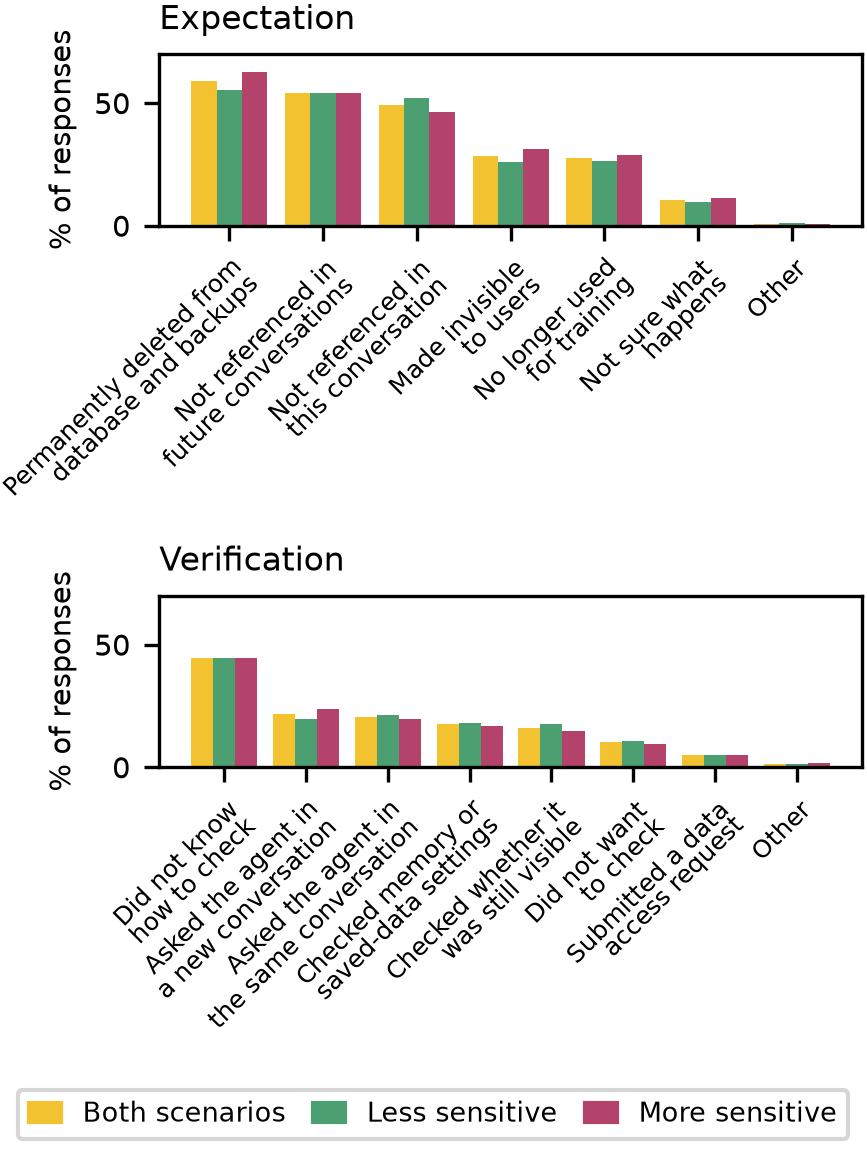
\includegraphics[width=\columnwidth,height=0.45\textheight,keepaspectratio]{figures/fig_expectation.png}
%     \caption{Expected deletion outcomes and reported verification strategies in LS, MS, and Pooled. The analysis includes 354 responses from 177 participants, with multiple selections allowed. Percentages are based on 177 participants within each scenario and 354 responses for Pooled results.}
%     \label{fig:expectation}
% \end{figure}


% \begin{figure*}[t]
%     \centering
%     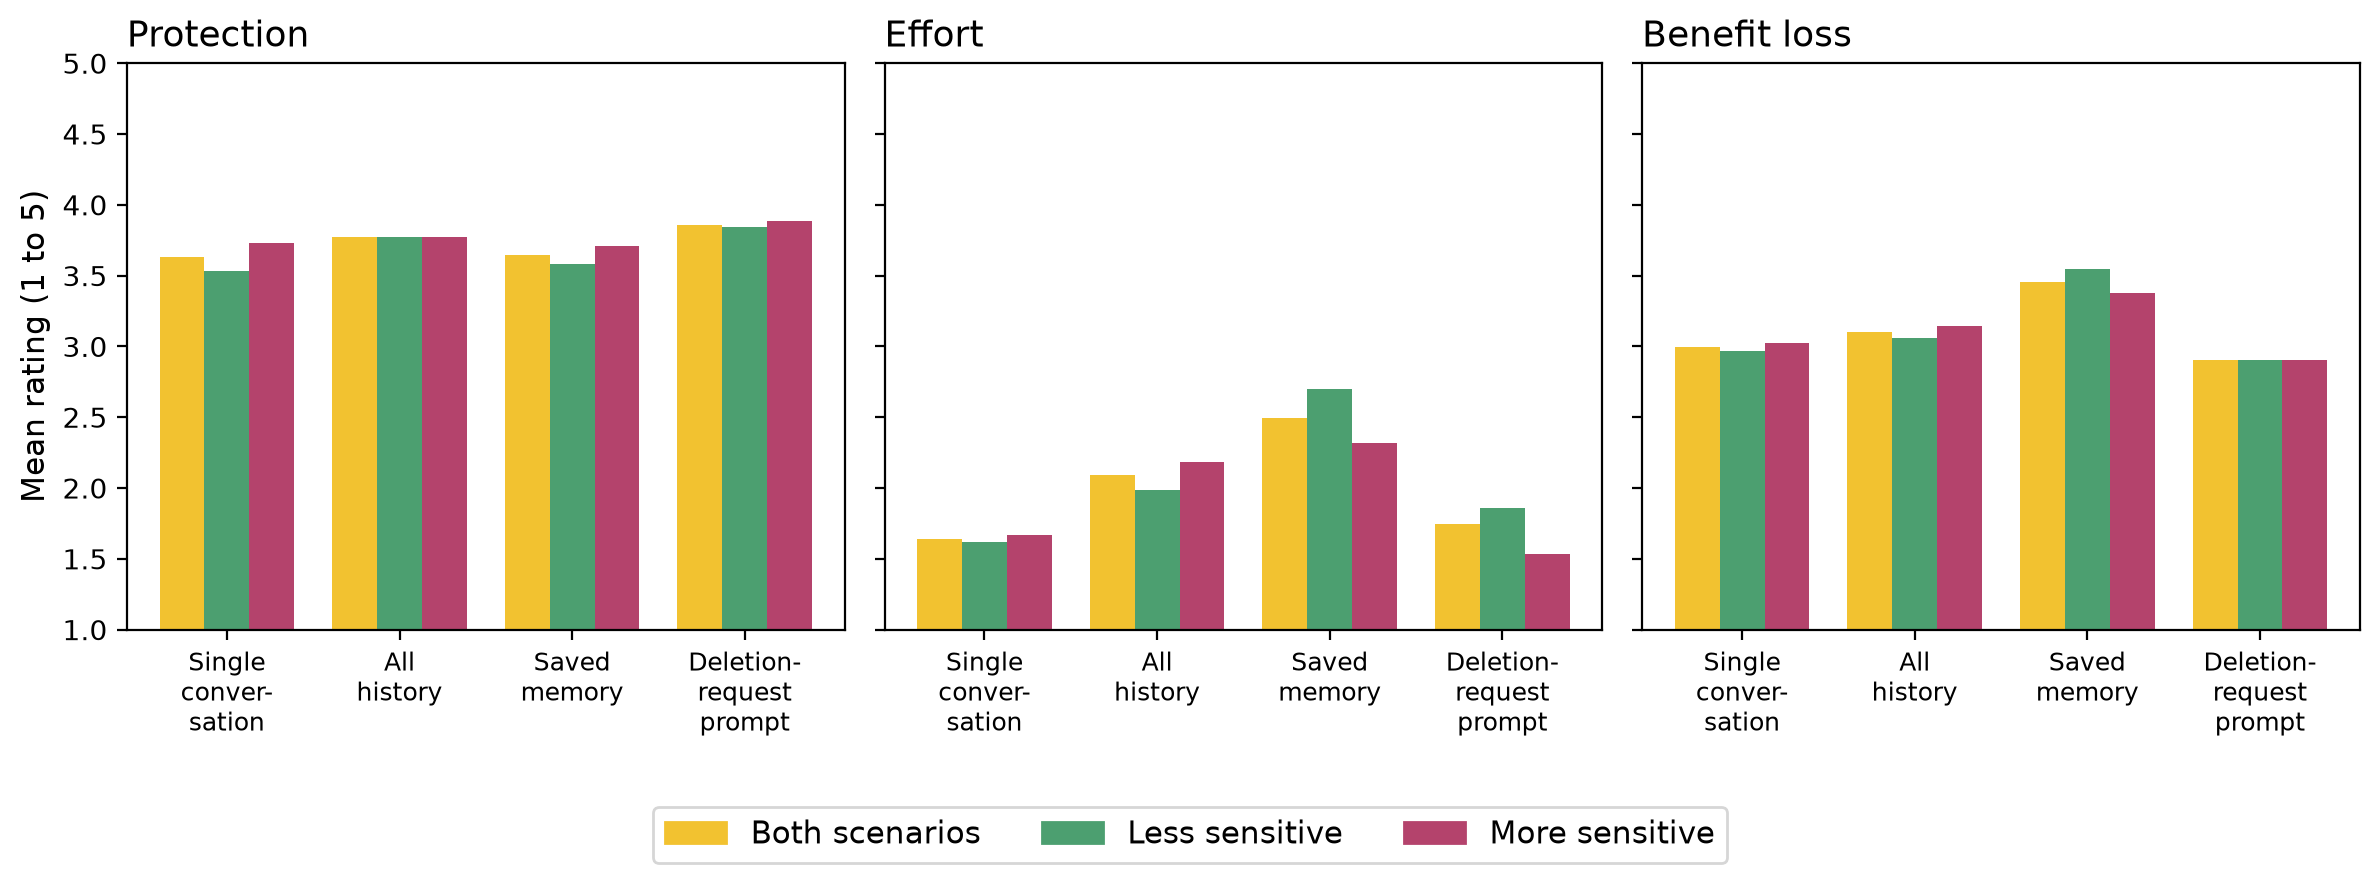
\includegraphics[width=0.94\textwidth]{figures/fig_scales.png}
%     \caption{Mean ratings of perceived privacy protection, effort, and potential loss of personalized benefits for the four most frequently selected deletion methods, shown separately for LS and MS and combined (Pooled). The analysis includes 317 responses from 105, 50, 30, and 29 participants, respectively. Ratings use five-point agreement scales.}
%     \label{fig:scales}
% \end{figure*}

% Many participants were uncertain how to verify deletion outcomes.
% %
% Across Pooled responses, 44.6\% indicated that they did not know how to verify deletion.
% %
% Reported verification strategies included asking the agent in the same or a new conversation (21\%--22\% of responses) and checking saved memories, settings, or the user interface (16\%--18\%).
% %
% Notably, among responses selecting a deletion-request prompt, 53.8\% (of 39 responses) indicated verification by asking the agent in the same conversation.
% %
% This suggests that users relying on conversational deletion requests may also rely on the agent's own responses as evidence that deletion succeeded.

% Participants also reported limitations in deletion feedback and experiences of information resurfacing.
% %
% Among the 177 participants, 42 (23.7\%) reported that an agent had referenced information they believed was deleted.
% %
% After previous deletion attempts, 41.2\% reported receiving a clear confirmation message, while 29.4\%--34.5\% reported vague acknowledgements or no feedback (multiple selections allowed).
% %
% Furthermore, 73 participants (41.2\%) wanted a breakdown specifying what information had been deleted and what might still be retained.
% %
% These findings highlight a gap between users' expectations of deletion and their ability to establish its outcome, motivating our subsequent post-deletion analysis (Section~\ref{sec:tech_analysis}).

% %
% \begin{takeawaybox}
% \textbf{Finding 2:} Participants commonly expected deletion methods to permanently remove their data, despite differences in the data locations these methods target. Perceived effort differed across methods, but expected deletion outcomes and perceived protection showed no significant differences. Many participants did not know how to verify deletion, and those selecting deletion-request prompts often relied on the agent itself for verification.
% \end{takeawaybox}

